\section{General Analysis Overview}

\section{Filtering}\label{sec:filtering}

For this analysis all final state particles should be detected.
After $\pi^0$ decay we are going to have 4 particles: electron, proton and two photons.
The particle identification methods are applied to select the exclusive event with at least one electron, proton and two photons. 


\section{Electron, Proton, and Photon}
Basic event builder cuts are utilized, then additional cuts are made that are common with the RGA Analysis note (\href{https://www.overleaf.com/project/5ea737720942930001ff5e9c}{overleaf link} and developed by Sangbaek Lee (sangbaek@mit.edu - \href{https://github.com/Sangbaek/analysis_code/tree/analysis/pid}{github code here}. For this analysis, both the central detector and forward detector are utilized for proton tracking. The forward tagger is also utilized for photon identification. 



\section{Neutral pion}
In addition to individual particle PID procedures the cut on the mass of two photons is applied:
\begin{itemize}
	\item $0.07<M_{\gamma\gamma}<0.2$ GeV
\end{itemize}
The pion is more thoroughly constrained by the exclusivity cuts, described in the next section.


\begin{figure}[hbt]
	\centering
	\includegraphics[page=6,width=0.6\textwidth]{Chapters/Ch4-BaseAnalysis/pid_figs/eppi0.exclusive.pdf}
	
	\caption{The distribution for mass of two photons $M_{\gamma\gamma}$}.
	\label{fig:ggmass}
	
	\centering
	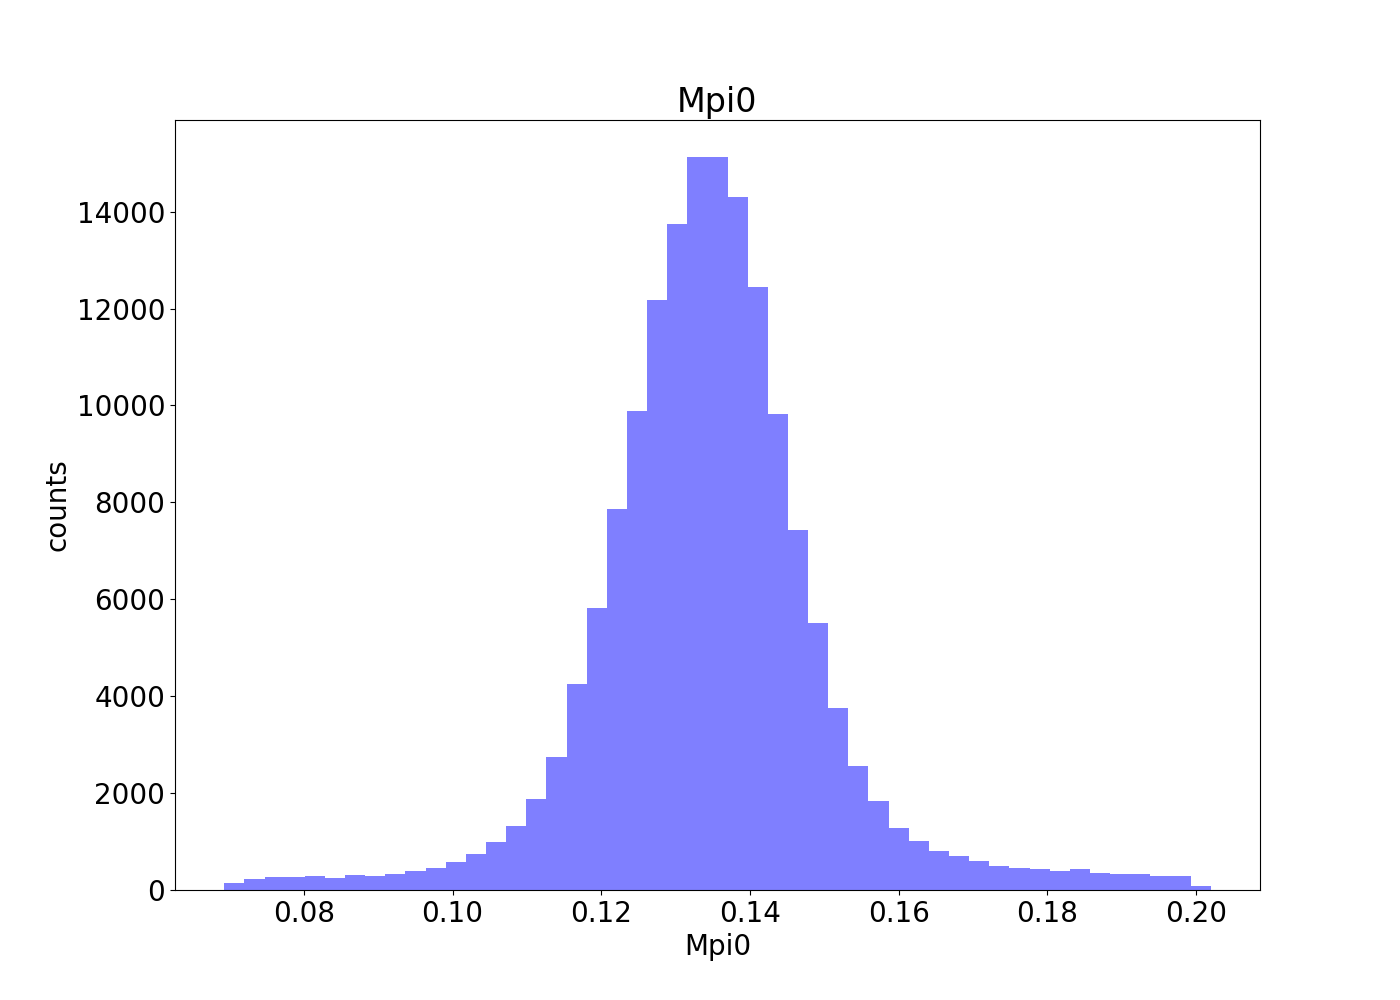
\includegraphics[width=0.6\textwidth]{Chapters/Ch4-BaseAnalysis/pid_figs/Mpi0.png}
	
	\caption{The distribution for mass of two photons after exclusivity cuts}.
	\label{fig:ggmass_after}
	
\end{figure}

\section{Decoding}\label{sec:decrec}
\section{Mom Smear}\label{sec:momsmear}

\section{Mom Corr}\label{sec:momcorr}

\Xsecs are theoretically interpreted as  the probability for a specific interaction to occur. They can be experimentally estimated by measuring the occurrence frequency relative to the total possible interaction opportunities. In general, the \xsec $\sigma$ can be expressed as \eqref{eq:basic_xsec} the number of measured events of interest $N_{meas}$ divided by the number of total interaction opportunities \Lumi. \Lumi is known as luminosity and is a product of only experimental parameters, such as the number of particles present and the experiment duration. 

\begin{equation} \label{eq:basic_xsec}
    \sigma = \frac{\counts}{\Lumi}
\end{equation}

Measuring the complete \xsec at once is not feasible, so instead estimates are made of the differential \xsec \eqref{eq:basic_diff_xsec}, which instead evaluates the probability for a specific interaction to occur in a differential region of phase space, $\frac{d\sigma}{d\Omega}$. Infinitesimal measurements are not possible, so events are counted over some small discretized generalized volume \textcolor{purple}{$\Delta \Omega$}. 

\begin{equation} \label{eq:basic_diff_xsec}
    \frac{d\sigma}{d\Omega} = \frac{ \counts} {\Lumi \textcolor{purple}{\Delta \Omega}}
\end{equation}

In practice, a number of correction terms need to be included to account for differences between experiment and theory. These correction terms, combined with the specifics of this analysis, yield the full experimental expression of the \xsec \eqref{eq:DVPiPCrossSection_exp}. 

     \begin{equation}\labelAndRemember{eq:DVPiPCrossSection_exp}
           { \frac{    d^4\sigma_{  ep \rightarrow ep'\pi^0}   } {dQ^2dx_Bdtd\phi_{\pi}} 
                =   \frac{ \textcolor{red}{ N(Q^2,x_B,t,\phi_{\pi})}} {\Lumiint \textcolor{purple}{ \Delta Q^2 \Delta x_B \Delta t \Delta \phi_{\pi}}} 
                \frac{1}{\textcolor{correctionfactors}{\epsilon_{acc} \delta_{RC} \delta_{Norm} Br(\pi^0\rightarrow\gamma\gamma)}}}
     \end{equation}      \myequations{DV$\pi$P Experimental Cross Section}

The terms on the right-hand side of this equation are: 
\begin{itemize}
\item \textcolor{red}{$N(Q^2,x_B,t,\phi_{\pi})$} - Number of events recorded in a given $Q^2$, $x_B$, $t$, $\phi_{\pi}$ bin.

\item \Lumiint - Integrated luminosity

\item \textcolor{purple}{$\Delta Q^2 \Delta x_B \Delta t \Delta \phi_{\pi}$} - These are the bin sizes or intervals for the variables $Q^2$, $x_B$, $t$, and $\phi_{\pi}$.

\item \textcolor{correctionfactors}{$\epsilon_{acc}$} - Acceptance correction, which is a combination of detector efficiency and geometrical acceptance, determined through simulations. 

\item \textcolor{correctionfactors}{$\delta_{RC}$} - Radiative correction factor

\item \textcolor{correctionfactors}{$\delta_{Norm}$} - Overall normalization factor

\item \textcolor{correctionfactors}{$Br(\pi^0\rightarrow\gamma\gamma)$} - Branching ratio of the decay of a neutral pion ($\pi^0$) into two photons ($\gamma\gamma$), which is most recently measured at 98.8131\%  \cite{Husek2019PreciseDecay}
\end{itemize}


\clearpage
\begin{figure}[!h]
    \centering
    \begin{tikzpicture}[
      node distance=2cm,
      startstop/.style={rectangle, rounded corners, minimum width=11cm, minimum height=1cm,text centered, draw=black, fill=red!30},
      io/.style={trapezium, trapezium left angle=70, trapezium right angle=110, minimum width=11cm, minimum height=1cm, text centered, draw=black, fill=blue!30},
      process/.style={rectangle, minimum width=11cm, minimum height=1cm, text centered, draw=black, fill=orange!30},
      arrow/.style={white,ultra thick,->,>=stealth},
      ]
    
      \node (start) [startstop] {Real or Simulated Detector Hits};
      \node (process1) [process, below of=start] {Reconstruction into Particle Tracks};
      \node (io1) [io, below of=process1] {Conversion to .HIPO format};
      \node (process2) [process, below of=io1] {Preliminary Fiducial Filtering};
      \node (io2) [io, below of=process2] {Conversion to .ROOT format};
      \node (process3) [process, below of=io2] {Preprocessing: Momentum Corrections and Smearing};
      \node (io3) [io, below of=process3] {Conversion to DataFrame Objects};
      \node (process4) [process, below of=io3] {\Xsec Calculation};
       
      \draw [arrow] (start) -- (process1);
      \draw [arrow] (process1) -- (io1);
      \draw [arrow] (io1) -- (process2);
      \draw [arrow] (process2) -- (io2);
      \draw [arrow] (io2) -- (process3);
      \draw [arrow] (process3) -- (io3);
      \draw [arrow] (io3) -- (process4);

    
      \begin{scope}[on background layer]
        \node[fit=(start)(process1)(io1), fill=mypurp, rounded corners, inner xsep=15pt, inner ysep=25pt, label={[xshift=-90pt, yshift=-20pt] north: \textcolor{white}{Step 0: Track Reconstruction} }] {};


        \node[fit=(process2)(io2), fill=darkblue, rounded corners, inner xsep=15pt, inner ysep=25pt, label={[xshift=-90pt, yshift=-20pt] north: \textcolor{white}{Step 1: Data Batching} }] {};


        \node[fit=(process3)(io3), fill=darkgreen, rounded corners, inner xsep=15pt, inner ysep=25pt, label={[xshift=-90pt, yshift=-20pt] north: \textcolor{white}{Step 2: Data Preparation} }] {};

        \node[fit=(process4), fill=darkred, rounded corners, inner xsep=15pt, inner ysep=25pt, label={[xshift=-90pt, yshift=-20pt] north: \textcolor{white}{Step 4: Analysis } }] {};

      \end{scope}
      
    \end{tikzpicture}
    \caption{High-level data processing flow}
    \label{fig:High-level data processing flow}
\end{figure}

\clearpage


Official Repo: https://github.com/robertej19/clas12DVPiP
         


For each kinematic bin the differential cross section can be written as:

\begin{equation}
    \sigma = \frac{N_{meas}}{L \epsilon}\frac{1}{\delta}
\end{equation}

Where $\frac{N_{meas}}{L}$ is the number of events from experiment normalized by the integrated luminosity before acceptance and radiatvie corrections. $\epsilon$ = $\frac{N^{RAD}_{rec}}{{N^{RAD}_{gen}}}$ is the acceptance correction and $\delta$ is the radiative correction.



$\delta$ can be obtained by using the following:

\begin{equation}
    \delta = \frac{N^{RAD}_{gen}}{N^{NORAD}_{gen}}
\end{equation}

$\delta$ and $\epsilon$ need to be properly calculated, but for a first pass we will ignore them so we have just



We can calculate the luminosity L through the following equation

\begin{equation}
    L = \frac{N_A l \rho Q_{FCUP}}{e}
\end{equation}

Where $N_A$ is Avogadro's constant, l is the length of the target,  $\rho$ is the density of the target (liquid hydrogen), $Q_{FCUP}$ is the charge collected on the Faraday cup, and e is the charge of the electron. The values of these quantities are (ignoring uncertainties on experimental quantities for the time being):\\

$N_A$ = 6.02214 x $10^{23}$\\
l = 5 cm\\
$\rho$ = 0.07 $g/cm^3$\\
e = 1.602 x $10^-19$ Coulombs\\
$Q_{FCUP}$ - this must be measured and obtained from analysis. Typical runs at CLAS12 have an accumulated beam charge of tens to hundreds of thousands of nanoCoulumbs. 

\section{Data Pre-Processing}
    \subsection{Energy Loss Corrections}
    \subsection{Momentum Corrections}
    \subsection{Simulation:Experiment Resolution Matching}
        \subsubsection{Kinematics Correction of Experimental Data}
        \subsubsection{Smearing Simulated Data}

\section{Particle Identification}

\section{Event Selection}
    \subsection{Rigid Event Selection}
    \subsection{Classifier Based Event Selection}
    \clearpage
\section{Exclusive distributions}\label{sec:eventselection}





\begin{wrapfigure}{r}{0.58\textwidth}
	\vspace*{-0.3cm}
	\includegraphics[page=10,width=0.97\linewidth]{Chapters/Ch4-BaseAnalysis/1_Exclusivity_Cuts/figures/eppi0.exclusive.pdf}
	\caption{MM$^2$ (epX) vs $\theta_X\pi$ 2D distribution.}
	\label{fig:MM2vsThetaXPi}
\end{wrapfigure}
After the selection of events with at least one electron, proton and two photons, it is time to take a look at the exclusive distributions.
The Fig.~\ref{fig:MM2vsThetaXPi} shows 2D distribution of MM$^2$ (epX) vs $\theta_{X\pi}$, where MM$^2$ (epX) is a missing mass squared of (epX) system and should have a peak near 0.0182 GeV$^2$, and $\theta_{X\pi}$ is an angle between expected and reconstructed pion.
The bright spot on the figure corresponds to the exclusive $ep\rightarrow~ep\pi^0$ events.
In order to reduce the background exclusivity cuts  need to be developed based on the conservation of energy and momentum.
The relevant 1D exclusive distributions are shown on the Fig.~\ref{fig:rawexclusive1} and \ref{fig:rawexclusive2}.

\begin{figure}[hbt]
	\centering
	\includegraphics[page=4,width=0.47\linewidth]{Chapters/Ch4-BaseAnalysis/1_Exclusivity_Cuts/figures/eppi0.exclusive.pdf}
	\includegraphics[page=5,width=0.47\linewidth]{Chapters/Ch4-BaseAnalysis/1_Exclusivity_Cuts/figures/eppi0.exclusive.pdf}

	\caption{Exclusive distributions for events with at least one electron, proton and two photons.}
	\label{fig:rawexclusive1}
\end{figure}

\begin{figure}[hbt]
	\centering
	\includegraphics[page=6,width=0.47\linewidth]{Chapters/Ch4-BaseAnalysis/1_Exclusivity_Cuts/figures/eppi0.exclusive.pdf}
	\includegraphics[page=8,width=0.47\linewidth]{Chapters/Ch4-BaseAnalysis/1_Exclusivity_Cuts/figures/eppi0.exclusive.pdf}
	
	\caption{Exclusive distributions for events with at least one electron, proton and two photons.}
	\label{fig:rawexclusive2}
\end{figure}

\subsection{Tight \texorpdfstring{$M_{\gamma\gamma} $} mass and transverse missing momenta cuts}

The first step is to use tighter $\gamma\gamma$ mass cut: $0.096<M_{\gamma\gamma}<0.168$ GeV, and take a look at the missing transverse momentum distributions (see Fig.~\ref{fig:ptdistributions}).
From momentum conservation law we expect transverse momentum to be zero, so we can apply cuts on $\Delta p_x$ and $\Delta p_y$ to further improve exclusive channel selection.
The cuts $|\Delta p_x|<0.2$ and $|\Delta p_y|<0.2$ correspond roughly to 4-5 $\sigma$.

\begin{figure}[hbt]
	\centering
	\includegraphics[page=24,width=0.47\linewidth]{Chapters/Ch4-BaseAnalysis/1_Exclusivity_Cuts/figures/eppi0.exclusive.pdf}
	\includegraphics[page=25,width=0.47\linewidth]{Chapters/Ch4-BaseAnalysis/1_Exclusivity_Cuts/figures/eppi0.exclusive.pdf}
	
	\caption{Exclusive distributions for events with at least one electron, proton and two photons.}
	\label{fig:ptdistributions}
\end{figure}

The exclusive distributions after tight $M_{\gamma\gamma}$ mass and transverse missing momenta cuts are shown on Fig.~\ref{fig:rawexclusive3} and display much stronger signal peaks on top of reduced background.

\begin{figure}[hbt]
	\centering
	\includegraphics[page=43,width=0.45\linewidth]{Chapters/Ch4-BaseAnalysis/1_Exclusivity_Cuts/figures/eppi0.exclusive.pdf}
	\includegraphics[page=44,width=0.45\linewidth]{Chapters/Ch4-BaseAnalysis/1_Exclusivity_Cuts/figures/eppi0.exclusive.pdf}
	
	\includegraphics[page=45,width=0.45\linewidth]{Chapters/Ch4-BaseAnalysis/1_Exclusivity_Cuts/figures/eppi0.exclusive.pdf}
    \includegraphics[page=47,width=0.45\linewidth]{Chapters/Ch4-BaseAnalysis/1_Exclusivity_Cuts/figures/eppi0.exclusive.pdf}

	\caption{Exclusive distributions after tight $M_{\gamma\gamma}$ mass and transverse missing momenta cuts .}
	\label{fig:rawexclusive3}
\end{figure}

\subsection{\texorpdfstring{$\theta_{X\pi}$} cut determination}

The cut on angle between expected and reconstructed pion is used in order to further reduce background.
To choose the value of the $\theta_{X\pi}$ cut the $MM^2(epX)$ distribution is analyzed at multiple $\theta_{X\pi}$ cut values and fit using gaussian+polynomial function as shown on Fig.~\ref{fig:mm2fordifferenttheta}.
From the fit we can estimate the number of good exclusive events (gaussian) and the number of background events (polynomial) and their dependence on $\theta_{X\pi}$ cut.
Fig.~\ref{fig:sigbgvsthetacutQ2} and~\ref{fig:sigbgvsthetacutxB} show the numbers of signal and background events as functions of $\theta_{X\pi}$ cut value for multiple bins in $Q^2$ and $x_B$.
These plots show that the cut $\theta_{X\pi}<2^\circ$ allows to select the most number of good events with the least background, and relaxing it beyond $2^\circ$ does not gain us any good exclusive events but increases background.


\begin{figure}[hbt]
	\centering
	\includegraphics[page=123,width=0.3\linewidth]{Chapters/Ch4-BaseAnalysis/1_Exclusivity_Cuts/figures/sigbg_eppi0.pdf}
	\includegraphics[page=125,width=0.3\linewidth]{Chapters/Ch4-BaseAnalysis/1_Exclusivity_Cuts/figures/sigbg_eppi0.pdf}
	\includegraphics[page=128,width=0.3\linewidth]{Chapters/Ch4-BaseAnalysis/1_Exclusivity_Cuts/figures/sigbg_eppi0.pdf}
	
	\includegraphics[page=130,width=0.3\linewidth]{Chapters/Ch4-BaseAnalysis/1_Exclusivity_Cuts/figures/sigbg_eppi0.pdf}
	\includegraphics[page=133,width=0.3\linewidth]{Chapters/Ch4-BaseAnalysis/1_Exclusivity_Cuts/figures/sigbg_eppi0.pdf}
	\includegraphics[page=135,width=0.3\linewidth]{Chapters/Ch4-BaseAnalysis/1_Exclusivity_Cuts/figures/sigbg_eppi0.pdf}
	
	\caption{$MM^2(epX)$ distributions for multiple $\theta_{X\pi}$ cut values.}
	\label{fig:mm2fordifferenttheta}
\end{figure}


\begin{figure}[hbt]
	\centering
	
	\includegraphics[width=0.32\linewidth,page=34]{Chapters/Ch4-BaseAnalysis/1_Exclusivity_Cuts/figures/sigbg_eppi0.pdf}
	\includegraphics[width=0.32\linewidth,page=51]{Chapters/Ch4-BaseAnalysis/1_Exclusivity_Cuts/figures/sigbg_eppi0.pdf}
	\includegraphics[width=0.32\linewidth,page=68]{Chapters/Ch4-BaseAnalysis/1_Exclusivity_Cuts/figures/sigbg_eppi0.pdf}
	
	\includegraphics[width=0.32\linewidth,page=85]{Chapters/Ch4-BaseAnalysis/1_Exclusivity_Cuts/figures/sigbg_eppi0.pdf}
	\includegraphics[width=0.32\linewidth,page=102]{Chapters/Ch4-BaseAnalysis/1_Exclusivity_Cuts/figures/sigbg_eppi0.pdf}
	\includegraphics[width=0.32\linewidth,page=119]{Chapters/Ch4-BaseAnalysis/1_Exclusivity_Cuts/figures/sigbg_eppi0.pdf}
	
	\caption{The numbers of signal (red markers) and background (black markers) events as functions of $\theta_{X\pi}$ cut value for multiple $Q^2$ bins.}
	\label{fig:sigbgvsthetacutQ2}
\end{figure}


\begin{figure}[hbt]
	\centering
	
	\includegraphics[width=0.32\linewidth,page=136]{Chapters/Ch4-BaseAnalysis/1_Exclusivity_Cuts/figures/sigbg_eppi0.pdf}
	\includegraphics[width=0.32\linewidth,page=153]{Chapters/Ch4-BaseAnalysis/1_Exclusivity_Cuts/figures/sigbg_eppi0.pdf}
	\includegraphics[width=0.32\linewidth,page=170]{Chapters/Ch4-BaseAnalysis/1_Exclusivity_Cuts/figures/sigbg_eppi0.pdf}
	
	\includegraphics[width=0.32\linewidth,page=187]{Chapters/Ch4-BaseAnalysis/1_Exclusivity_Cuts/figures/sigbg_eppi0.pdf}
	\includegraphics[width=0.32\linewidth,page=204]{Chapters/Ch4-BaseAnalysis/1_Exclusivity_Cuts/figures/sigbg_eppi0.pdf}
	
	\caption{The numbers of signal (red markers) and background (black markers) events as functions of $\theta_{X\pi}$ cut value for multiple $x_B$ bins.}
	\label{fig:sigbgvsthetacutxB}
\end{figure}

\clearpage

\subsection{Final exclusivity cuts}

The list of final exclusive cuts is following:
\begin{itemize}
	\item $\Delta p_x<0.2$ GeV
	\item $\Delta p_y<0.2$ GeV
	\item $\theta_{X\pi}<2^\circ$
	\item $0.096<M_{\gamma\gamma}<0.168$ GeV
	\item $MM^2(epX)<0.5$ GeV$^2$
\end{itemize}

Exclusive distributions after all exclusivity cut except $MM^2(epX)<0.5$ GeV are shown on Fig.~\ref{fig:finalexclusive}

\begin{figure}[hbt]
	\centering
	
	\includegraphics[page=82,width=0.32\linewidth]{Chapters/Ch4-BaseAnalysis/1_Exclusivity_Cuts/figures/eppi0.exclusive.pdf}
	\includegraphics[page=83,width=0.32\linewidth]{Chapters/Ch4-BaseAnalysis/1_Exclusivity_Cuts/figures/eppi0.exclusive.pdf}
	\includegraphics[page=84,width=0.32\linewidth]{Chapters/Ch4-BaseAnalysis/1_Exclusivity_Cuts/figures/eppi0.exclusive.pdf}
	\caption{Exclusive distributions after all exclusivity cuts .}
	\label{fig:finalexclusive}
\end{figure}







To arrive at a DVEP candidate event, we do the following


Code flow:

Consider a directory with n hipo files. For each hipo file, do the following.

Read each file event by event, and do the following

Check that the event has the proper databanks, and if not, go to teh next event.

Get a list of all the electrons*, protons*, and photons* in the event

*= links to most up to date PID methods

for every electron in the event (always only one, at least in the skims, but not held to be one) do the following
For every proton in the event, do the following

Calculate some basic quantities and fill histograms

for every permutation of pairs of photons in the event, do the following

calculate various kinematic quantities, and pass to see if creates a viable pion* and a viable DVEP event*

if so, fill relevant histograms and count as a DVEP event, otherwise skip to next event

viable pion: 
pion mass betwen 100 and 180 MeV
pion momentum greater than 1.5 GeV
angle (theta) between each photon and the electron to be greater than 8 degrees

viable DVEP event:
Q2 greater than 1
W greater than 2
difference between theta of missing 4-momentum and reconstructed pion less than 2 degrees
difference between missing X px and py 300 MeV each or less
Difference in missing mass squared between pion and X less than 1 GeV ** make sure this is right
difference in missing energy and X less than 1 GeV **make sure this is right

**photon cuts:
pid 22, status > 2000 (in FD or CD, not ftagger)
momentum greater than 400 MeV each

**proton cuts: pid 2212

**electron cuts: pid==1 and status < 0(negative particle


\iffalse
\begin{wrapfigure}{r}{0.58\textwidth}
	\vspace*{-0.3cm}
	\includegraphics[page=10,width=0.97\linewidth]{figures/eppi0.exclusive.pdf}
	\caption{MM$^2$ (epX) vs $\theta_X\pi$ 2D distribution.}
	\label{fig:MM2vsThetaXPi}
\end{wrapfigure}
After the selection of events with at least one electron, proton and two photons, it is time to take a look at the exclusive distributions.
The Fig.~\ref{fig:MM2vsThetaXPi} shows 2D distribution of MM$^2$ (epX) vs $\theta_{X\pi}$, where MM$^2$ (epX) is a missing mass squared of (epX) system and should have a peak near 0.0182 GeV$^2$, and $\theta_{X\pi}$ is an angle between expected and reconstructed pion.
The bright spot on the figure corresponds to the exclusive $ep\rightarrow~ep\pi^0$ events.
In order to reduce the background exclusivity cuts  need to be developed based on the conservation of energy and momentum.
The relevant 1D exclusive distributions are shown on the Fig.~\ref{fig:rawexclusive1} and \ref{fig:rawexclusive2}.

\begin{figure}[hbt]
	\centering
	\includegraphics[page=4,width=0.47\linewidth]{figures/eppi0.exclusive.pdf}
	\includegraphics[page=5,width=0.47\linewidth]{figures/eppi0.exclusive.pdf}

	\caption{Exclusive distributions for events with at least one electron, proton and two photons.}
	\label{fig:rawexclusive1}
\end{figure}

\begin{figure}[hbt]
	\centering
	\includegraphics[page=6,width=0.47\linewidth]{figures/eppi0.exclusive.pdf}
	\includegraphics[page=8,width=0.47\linewidth]{figures/eppi0.exclusive.pdf}
	
	\caption{Exclusive distributions for events with at least one electron, proton and two photons.}
	\label{fig:rawexclusive2}
\end{figure}

\subsection{Tight $M_{\gamma\gamma}$ mass and transverse missing momenta cuts}

The first step is to use tighter $\gamma\gamma$ mass cut: $0.096<M_{\gamma\gamma}<0.168$ GeV, and take a look at the missing transverse momentum distributions (see Fig.~\ref{fig:ptdistributions}).
From momentum conservation law we expect transverse momentum to be zero, so we can apply cuts on $\Delta p_x$ and $\Delta p_y$ to further improve exclusive channel selection.
The cuts $|\Delta p_x|<0.2$ and $|\Delta p_y|<0.2$ correspond roughly to 4-5 $\sigma$.

\begin{figure}[hbt]
	\centering
	\includegraphics[page=24,width=0.47\linewidth]{figures/eppi0.exclusive.pdf}
	\includegraphics[page=25,width=0.47\linewidth]{figures/eppi0.exclusive.pdf}
	
	\caption{Exclusive distributions for events with at least one electron, proton and two photons.}
	\label{fig:ptdistributions}
\end{figure}

The exclusive distributions after tight $M_{\gamma\gamma}$ mass and transverse missing momenta cuts are shown on Fig.~\ref{fig:rawexclusive3} and display much stronger signal peaks on top of reduced background.

\begin{figure}[hbt]
	\centering
	\includegraphics[page=43,width=0.45\linewidth]{figures/eppi0.exclusive.pdf}
	\includegraphics[page=44,width=0.45\linewidth]{figures/eppi0.exclusive.pdf}
	
	\includegraphics[page=45,width=0.45\linewidth]{figures/eppi0.exclusive.pdf}
    \includegraphics[page=47,width=0.45\linewidth]{figures/eppi0.exclusive.pdf}

	\caption{Exclusive distributions after tight $M_{\gamma\gamma}$ mass and transverse missing momenta cuts .}
	\label{fig:rawexclusive3}
\end{figure}

\subsection{$\theta_{X\pi}$ cut determination}

The cut on angle between expected and reconstructed pion is used in order to further reduce background.
To choose the value of the $\theta_{X\pi}$ cut the $MM^2(epX)$ distribution is analyzed at multiple $\theta_{X\pi}$ cut values and fit using gaussian+polynomial function as shown on Fig.~\ref{fig:mm2fordifferenttheta}.
From the fit we can estimate the number of good exclusive events (gaussian) and the number of background events (polynomial) and their dependence on $\theta_{X\pi}$ cut.
Fig.~\ref{fig:sigbgvsthetacutQ2} and~\ref{fig:sigbgvsthetacutxB} show the numbers of signal and background events as functions of $\theta_{X\pi}$ cut value for multiple bins in $Q^2$ and $x_B$.
These plots show that the cut $\theta_{X\pi}<2^\circ$ allows to select the most number of good events with the least background, and relaxing it beyond $2^\circ$ does not gain us any good exclusive events but increases background.


\begin{figure}[hbt]
	\centering
	\includegraphics[page=123,width=0.3\linewidth]{figures/sigbg_eppi0.pdf}
	\includegraphics[page=125,width=0.3\linewidth]{figures/sigbg_eppi0.pdf}
	\includegraphics[page=128,width=0.3\linewidth]{figures/sigbg_eppi0.pdf}
	
	\includegraphics[page=130,width=0.3\linewidth]{figures/sigbg_eppi0.pdf}
	\includegraphics[page=133,width=0.3\linewidth]{figures/sigbg_eppi0.pdf}
	\includegraphics[page=135,width=0.3\linewidth]{figures/sigbg_eppi0.pdf}
	
	\caption{$MM^2(epX)$ distributions for multiple $\theta_{X\pi}$ cut values.}
	\label{fig:mm2fordifferenttheta}
\end{figure}


\begin{figure}[hbt]
	\centering
	
	\includegraphics[width=0.32\linewidth,page=34]{figures/sigbg_eppi0.pdf}
	\includegraphics[width=0.32\linewidth,page=51]{figures/sigbg_eppi0.pdf}
	\includegraphics[width=0.32\linewidth,page=68]{figures/sigbg_eppi0.pdf}
	
	\includegraphics[width=0.32\linewidth,page=85]{figures/sigbg_eppi0.pdf}
	\includegraphics[width=0.32\linewidth,page=102]{figures/sigbg_eppi0.pdf}
	\includegraphics[width=0.32\linewidth,page=119]{figures/sigbg_eppi0.pdf}
	
	\caption{The numbers of signal (red markers) and background (black markers) events as functions of $\theta_{X\pi}$ cut value for multiple $Q^2$ bins.}
	\label{fig:sigbgvsthetacutQ2}
\end{figure}


\begin{figure}[hbt]
	\centering
	
	\includegraphics[width=0.32\linewidth,page=136]{figures/sigbg_eppi0.pdf}
	\includegraphics[width=0.32\linewidth,page=153]{figures/sigbg_eppi0.pdf}
	\includegraphics[width=0.32\linewidth,page=170]{figures/sigbg_eppi0.pdf}
	
	\includegraphics[width=0.32\linewidth,page=187]{figures/sigbg_eppi0.pdf}
	\includegraphics[width=0.32\linewidth,page=204]{figures/sigbg_eppi0.pdf}
	
	\caption{The numbers of signal (red markers) and background (black markers) events as functions of $\theta_{X\pi}$ cut value for multiple $x_B$ bins.}
	\label{fig:sigbgvsthetacutxB}
\end{figure}

\clearpage

\subsection{Final exclusivity cuts}

The list of final exclusive cuts is following:
\begin{itemize}
	\item $\Delta p_x<0.2$ GeV
	\item $\Delta p_y<0.2$ GeV
	\item $\theta_{X\pi}<2^\circ$
	\item $0.096<M_{\gamma\gamma}<0.168$ GeV
	\item $MM^2(epX)<0.5$ GeV$^2$
\end{itemize}

Exclusive distributions after all exclusivity cut except $MM^2(epX)<0.5$ GeV are shown on Fig.~\ref{fig:finalexclusive}

\begin{figure}[hbt]
	\centering
	
	\includegraphics[page=82,width=0.32\linewidth]{figures/eppi0.exclusive.pdf}
	\includegraphics[page=83,width=0.32\linewidth]{figures/eppi0.exclusive.pdf}
	\includegraphics[page=84,width=0.32\linewidth]{figures/eppi0.exclusive.pdf}
	\caption{Exclusive distributions after all exclusivity cuts .}
	\label{fig:finalexclusive}
\end{figure}

\fi
    \section{Cuts}

To arrive at a DVEP candidate event, we do the following


Code flow:

Consider a directory with n hipo files. For each hipo file, do the following.

Read each file event by event, and do the following

Check that the event has the proper databanks, and if not, go to teh next event.

Get a list of all the electrons*, protons*, and photons* in the event

*= links to most up to date PID methods

for every electron in the event (always only one, at least in the skims, but not held to be one) do the following
For every proton in the event, do the following

Calculate some basic quantities and fill histograms

for every permutation of pairs of photons in the event, do the following

calculate various kinematic quantities, and pass to see if creates a viable pion* and a viable DVEP event*

if so, fill relevant histograms and count as a DVEP event, otherwise skip to next event

viable pion: 
pion mass betwen 100 and 180 MeV
pion momentum greater than 1.5 GeV
angle (theta) between each photon and the electron to be greater than 8 degrees

viable DVEP event:
Q2 greater than 1
W greater than 2
difference between theta of missing 4-momentum and reconstructed pion less than 2 degrees
difference between missing X px and py 300 MeV each or less
Difference in missing mass squared between pion and X less than 1 GeV ** make sure this is right
difference in missing energy and X less than 1 GeV **make sure this is right

**photon cuts:
pid 22, status > 2000 (in FD or CD, not ftagger)
momentum greater than 400 MeV each

**proton cuts: pid 2212

**electron cuts: pid==1 and status < 0(negative particle
    
\section{Luminosity}
    \section{Luminosity} \label{sec:luminosity}

The strategy to calculate the luminosity is as follows:\\

 - For each run, retrieve a measure of how much beam passed through the target, I believe in the case of CLAS12 using the Faraday cup to measure beam charge
    - sum the beam charge over all runs being considered and include any relevant corrections factors
    - multiply this by target length, density, etc. to get the integrated luminosity
    - use this value to calculate cross sections.


Compare integrated luminosity of CLAS6 to CLAS12 (in 2011 analysis note)


Implementation:
The bank \texttt{REC::Event} has an object \texttt{beamCharge}, in nanoCoulombs, which is described in the \texttt{DST} as ``beam charge integrated from the beginning of the run to the most recent reading of the gated Faraday Cup scaler in \texttt{RAW::scaler}, with slope/offset conversion to charge from CCDB. Note, this value will be zero in each file until the first scaler reading in that file.''. This is the (un?)gated beam charge. 



This can be accessed via:

\begin{lstlisting}
	def banknames = ['REC::Event','REC::Particle','REC::Cherenkov','REC::Calorimeter','REC::Traj','REC::Track','REC::Scintillator']

	if(banknames.every{event.hasBank(it)}) {
		def (evb,partb,cc,ec,traj,trck,scib) = banknames.collect{event.getBank(it)}
def fcupBeamCharge = evb.getFloat('beamCharge',0)
\end{lstlisting}

    According to \href{https://clas12.discourse.group/t/accessing-beam-charge-information/239}{this} we might need to use tag=1 RAW::scaler::fcupgated instead of REC::Event::beamCharge
    

The beam charge needs to be converted to integrated luminosity, which can be done as follows:

Luminosity: Events are not necessarily time ordered, need to take largest value minus smallest value  


Luminosity is calculated according to equation \ref{lumieq}
 \begin{equation}\label{lumieq}
            \Lumi = \frac{N_A l \rho Q_{FCUP}}{e}
\end{equation}

The terms in equation \ref{lumieq} are as tabulated in table \ref{lumitable}. The accumulated charge on the Faraday cup is calculated by taking difference between the maximum and minimum values of beamQ for each run, and then summing these values. The luminosity determined for the fall 2018 inbending run was 5.5E+40 cm$^{-2}$ and the fall 2018 outbending run was 4.65E+40 cm$^{-2}$

\begin{table}[h]
    \centering
    \begin{tabular}{rcc}
         %& Heading 1 & Heading 2 \\\hline
        Quantity &  & CLAS12 Value \\\hline
       Avogadro's Number &  N$_A$  & $6x10^{23}$ \\
        Electron Charge &e  &  $1.6x10^{-19}$ \\
        Target Length &l &  5 cm \\
        Target Density &$\rho$  &  0.07 $g/cm^3$ (LH2) \\
        Charge on Faraday Cup & $Q_{FCUP}$ &  In data\\
    \end{tabular}
\caption{Terms of Luminosity Equation}
\end{table}\label{lumitable}

    
\section{Configuration and Kinematics}

\section{Binning}

\section{Acceptance Correction}

\section{Radiative Corrections}

\section{Binning Corrections}

\section{Overall Normalization Corrections}

\section{Error Analysis}

